\documentclass[12pt, a4paper]{book}

\usepackage[T1]{fontenc}
\usepackage{ucs}
\usepackage[utf8x]{inputenc}
\usepackage[english, greek]{babel}

\usepackage[version=3]{mhchem}

%Paragraph
%\usepackage{indentfirst}
\usepackage{parskip}
\setlength{\parskip}{.5cm}

%Graphics
\usepackage{graphicx}
\usepackage{caption}
\usepackage{subcaption}
\usepackage{float}
\usepackage{wrapfig}
\usepackage[labelfont=bf]{caption}
\DeclareGraphicsExtensions{.pdf,.png,.jpg}

%Source code
\usepackage{listings} %source code

%Tables
\usepackage{booktabs}
%\usepackage{hhline}

%Page
\usepackage{fullpage}

%Hyper reference
\usepackage[unicode]{hyperref}

%Math
\usepackage{amsmath, amsthm, amssymb}
%\usepackage{gfsartemisia-euler}

%URL
\usepackage{url}

%Footnote
\usepackage{threeparttablex}
%\usepackage{footnote}

%Commands
\newcommand{\eng}[1]{\selectlanguage{english}#1\selectlanguage{greek}}
\newcommand{\gre}[1]{\selectlanguage{greek}#1\selectlanguage{english}}

\newcommand{\en}{\selectlanguage{english}}
\newcommand{\gr}{\selectlanguage{greek}}

\newcommand{\norm}[1]{\left\lVert#1\right\rVert}

\begin{document}

\tableofcontents

%%%%%%%%%%%%%%%%%%%%%%%%%%%%%%%%%%%%%%%%%%%%%%%%%%%%%%%%%%%%%%%%%%%%%%%%%%%%%%%%
\chapter{Συσκευή Καταγραφής Κίνησης}

Στο παρόν κεφάλαιο θα γίνει μια σύντομη ανασκόπηση των χαρακτηριστικών του αισθητήρα. Θα εξηγήσουμε πως δουλεύει ο αλγόριθμος ανίχνευσης του σκελετού και πώς μπορούμε να έχουμε πρόσβαση στις τροχαίες των αρθρώσεων που είναι απαραίτητες για να γίνει η καταγραφή της κίνησης. Θα αναφέρουμε εναλλακτικά εργαλεία που μπορεί να χρησιμοποιήσει κανείς και θα κάνουμε μια σύγκριση μεταξύ τους. Έπειτα θα περάσουμε στο κομμάτι των μετρήσεων και στο πώς μπορούμε να βελτιώσουμε την ποιότητα τους. Τέλος θα γίνει επίδειξη του συστήματος που υλοποιήθηκε για την καταγραφή της βάδισης.

%%%%%%%%%%%%%%%%%%%%%%%%%%%%%%%%%%%%%%%%%%%%%%%%%%%%%%%%%%%%%%%%%%%%%%%%%%%%%%%%
\section{Αισθητήρας}

Ο αισθητήρας της \eng{Microsoft} που πρωτοεμφανίστηκε το 2009 ήταν μια καινοτομία που αρχικά προοριζόταν για την βιομηχανία των παιχνιδιών, αλλά λόγω των πολύ μεγάλων δυνατοτήτων και σχετικά χαμηλής τιμής σύντομα μπήκε στο στόχαστρο της ανοιχτής κοινότητας η οποία κατάφερε να το \lq χακάρει\rq  και να διαθέσει το πρώτο \eng{API} για πρόσβαση στην συσκευή. Με αποτέλεσμα μετά από λίγο καιρό να βγάλει και η \eng{Microsoft} το αντίστοιχο \eng{API}.

%%%%%%%%%%%%%%%%%%%%%%%%%%%%%%%%%%%%%%%%%%%%%%%%%%%%%%%%%%%%%%%%%%%%%%%%%%%%%%%%
\subsection{Χαρακτηριστικά}

Το \eng{Kinect} βασίζεται σε τεχνολογία λογισμικού η οποία έχει αναπτυχθεί από την \eng{Rare}, θυγατρική της \eng{Microsoft}. Η τεχνολογία της κάμερας αναπτύχθηκε από την ισραηλινή εταιρία \eng{PrimeSense} , η οποία ανέπτυξε ένα σύστημα που μπορεί να ερμηνεύσει συγκεκριμένες χειρονομίες, καθιστώντας δυνατόν τον έλεγχο ηλεκτρονικών συσκευών χωρίς κάποια άλλη συσκευή εισόδου, αλλά μόνο χειρονομίες σώματος. Για να γίνει αυτό δυνατόν χρησιμοποιείτε μια υπέρυθρη κάμερα, ένας προβολέας υπερύθρων και ένα ειδικό μικροτσίπ για να παρακολουθεί την κίνηση των αντικειμένων και τα άτομα σε τρεις διαστάσεις. Αυτό το σύστημα \eng{3D scanner} που ονομάζεται \eng{Light Coding} χρησιμοποιεί μια παραλλαγή εικόνας (χάρτης βάθους) η οποία μπορεί να αναπαρασταθεί σε τρισδιάστατο χώρο. Η συσκευή διαθέτει μία \eng{RGB} (8\-\eng{bits} των τριών καναλιών) κάμερα, αισθητήρα βάθους (11\-\eng{bits} μέχρι 2048 διακριτές στάθμες) και \eng{multi-array} μικρόφωνο και είναι ικανό να παρέχει πλήρη σωματική απεικόνιση \eng{3D}, καταγραφή κίνησης, αναγνώριση προσώπου και δυνατότητες αναγνώρισης φωνής όπως φαίνεται στην εικόνα \ref{fig:kinect-characteristics}.

\begin{figure}[H]
    \centering
    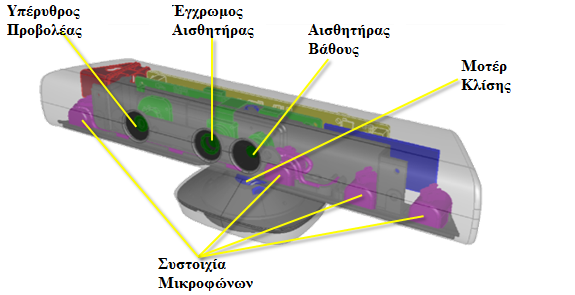
\includegraphics[width=.8\textwidth]{kinect/fig/kinect-characteristics.png}
    \caption{Ο αισθητήρας}
    \label{fig:kinect-characteristics}
\end{figure}

Ο αισθητήρας βάθους αποτελείται από ένα υπέρυθρο προβολέα λέιζερ σε συνδυασμό με ένα μονόχρωμη αισθητήρα \eng{CMOS}, ο οποίος καταγράφει δεδομένα βίντεο σε \eng{3D} κάτω από οποιεσδήποτε συνθήκες φωτισμού. Η τεχνολογία του λογισμικού επιτρέπει την προηγμένη αναγνώριση χειρονομιών, αναγνώριση προσώπου και αναγνώριση φωνής. Σύμφωνα με τις πληροφορίες που παρέχονται στους εμπόρους λιανικής πώλησης, το \eng{Kinect} είναι σε θέση να εντοπίζει ταυτόχρονα έως έξι άτομα. Ο χάρτης βάθους που δημιουργείτε από τον αισθητήρα βάθους, είναι στην ουσία μία εικόνα, η οποία χρησιμοποιώντας διαφορετικές αποχρώσεις χρώματος από λευκό έως μπλε ανάλογα με την απόσταση τον αντικειμένων που 'βλέπει'. Αν σκεφτεί κανείς το μικρό σχετικό κόστος με τις δυνατότητες και την πληροφορία που σου παρέχει το \eng{Kinect} μπορεί κανείς να το συνδυάσει και να δημιουργήσει πολύ ενδιαφέρουσες εφαρμογές \cite{jean13}. Στον πίνακα \ref{tab:sensor-characteristics} συνοψίζονται τα βασικά τεχνικά χαρακτηριστικά λειτουργίας.

\begin{center}
    \begin{tabular}{ll}
        \toprule
        % after \\: \hline or \cline{col1-col2} \cline{col3-col4} ...
        \multicolumn{2}{c}{Χαρακτηριστικά} \\
        \midrule
        Ανάλυση & $1280\times 960, \quad 1024\times 768,$ \\
          & $640\times 480, \quad 320\times 240$ \\
        Υπέρυθρη αόρατη δέσμη & $0.4m$ έως $3.5m$ \\
        Χάρτης βάθους, \eng{RGB} ροή δεδομένων & μέχρι 30 \eng{FPS} \\
        Κάθετης κλίσης & $\pm 27^{o}$ \\
        Κάθετο πεδίο ορατότητας & $43.5^{ο}$ \\
        Οριζόντιο πεδίο ορατότητας & $57^{ο}$ \\
        \bottomrule
    \end{tabular}
    \captionof{table}{Χαρακτηριστικά της συσκευής}
    \label{tab:sensor-characteristics}
\end{center}

\begin{figure}[H]
    \centering
    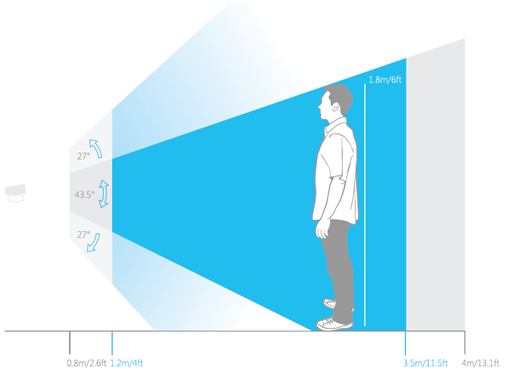
\includegraphics[width=.9\textwidth]{kinect/fig/kinect-operation-mode.png}
    \caption{Περιοχή λειτουργίας}
    \label{fig:kinect-operation-mode}
\end{figure}

%%%%%%%%%%%%%%%%%%%%%%%%%%%%%%%%%%%%%%%%%%%%%%%%%%%%%%%%%%%%%%%%%%%%%%%%%%%%%%%%
\subsection{Αλγόριθμος Ανίχνευση Σκελετού}

Η υλοποίηση ενός αλγορίθμου ανίχνευσης του σκελετού είναι ένα δύσκολο κομμάτι που σχετίζεται με το κλάδο της υπολογιστικής όρασης \cite{mubarak97}, αλλά και άλλων κλάδων. Η ανίχνευση του σκελετού έχει μελετηθεί σε βάθος \cite{thomas00, poppe07} στο παρελθών. Με την δυνατότητα στερεοσκοπικής όρασης, αλλά και τον στόχο να αλληλεπιδρά με τον άνθρωπο η ομάδα έρευνας της \eng{Microsoft} υλοποιείσαι εσωτερικά έναν αλγόριθμο εκτίμησης της στάσης του ανθρώπου και την θέση των αρθρώσεων \cite{shotton11} με κριτήρια, τόσο στην ακρίβεια των αποτελεσμάτων, όσο και στην ταχύτητα για εφαρμογές πραγματικού χρόνο.

\begin{figure}[H]
    \centering
    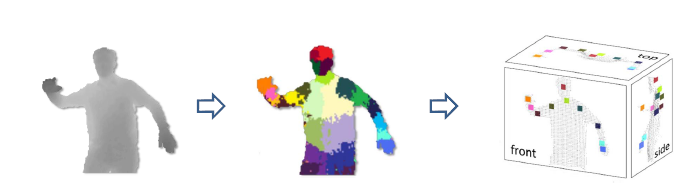
\includegraphics[width=.9\textwidth]{kinect/fig/kinect-skeleton-algorithm.png}
    \caption{Διαδικασία εξαγωγής της θέσης των αρθρώσεων}
    \label{fig:kinect-skeleton-algorithm}
\end{figure}

Ο αλγόριθμος αρχικά εκτιμά τις θέσεις των αρθρώσεων με βάση την εικόνας βάθους μαντεύοντας για κάθε εικονοστοιχείο πόσο πιθανό είναι να βρίσκεται μια άρθρωση στο συγκεκριμένο σημείο δίνοντας ένα επίπεδο εμπιστοσύνης. Έπειτα επιλέγει το σκελετό που είναι πιο πιθανό να δώσει αυτές τις ετικέτες στις αρθρώσεις για τα επίπεδα εμπιστοσύνης. Αλλά πριν μπορέσει να γίνει αυτό, ο αλγόριθμος πρέπει να κάνει ακριβείς εικασίες για τη θέση των αρθρώσεων. Αρχικά, συλλέχθηκαν εικόνες βάθους για τις οποίες ήταν ήδη γνωστή η θέση των αρθρώσεων για να μπορεί να γίνει η εκπαίδευση του αλγορίθμου και συντέθηκα επιπλέον εικόνες με διαφορετικά χαρακτηριστικά σώματος όπως φαίνεται στην εικόνα \ref{fig:kinect-data-synthesis}. Η αναγνώριση βασίζεται στην θεωρία των τυχαίων δέντρων απόφασης (\eng{randomized decision forest}).

\begin{figure}[H]
    \centering
    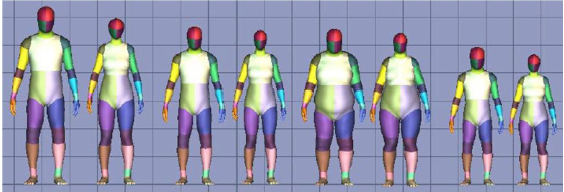
\includegraphics[width=.9\textwidth]{kinect/fig/kinect-data-synthesis.png}
    \caption{Σύνθεσης των εικόνων βάθους για την εκπαίδευση του αλγορίθμου}
    \label{fig:kinect-data-synthesis}
\end{figure}

Το πρόβλημα είναι πολύ δύσκολο και εξαρτάται από πολλούς παράγοντες, όπως είναι το φως, η διαφοροποίηση των ανθρώπων, οι ποικίλες στάσεις, το χρώμα, το δίσημο και από παρεμπόδιση τμημάτων του σώματος που δεν είναι ορατά στον αισθητήρα (\eng{occlusion}). Ο αλγόριθμος επιτυγχάνει πολύ υψηλά ποσοστά ανίχνευσης με μεγάλη ακρίβεια. Είναι ταχύτατος γιατί από την φύση του μπορεί να εκτελεστεί παράλληλα, με αποτέλεσμα η υλοποίηση του να γίνει στο υλικό εσωτερικά και όχι από λογισμικό.

Αυτό που απασχολεί τον χρήστη είναι πως θα μπορέσει να έχει πρόσβαση σε αυτή την πληροφορία. Το πρόβλημα είναι απλό, αφού το \eng{API} διαθέτει συναρτήσεις που σου παρέχουν την δυνατότητα. Ανάλογα με την βιβλιοθήκη που θα χρησιμοποιήσει κανείς για να έχει πρόσβαση στον αισθητήρα πρέπει να μελετήσει τις δυνατότητες που του περεχεί, αλλά και την ευκολία για την ρύθμιση της συσκευής.

%%%%%%%%%%%%%%%%%%%%%%%%%%%%%%%%%%%%%%%%%%%%%%%%%%%%%%%%%%%%%%%%%%%%%%%%%%%%%%%%
\section{Εργαλεία}

Υπάρχουν πολλές εναλλακτικές λύσεις για το πιο εργαλείο μπορεί να χρησιμοποιηθεί για πρόσβαση στα δεδομένα που σου παρέχει το Kinect. Παρακάτω θα αναφερθούν δύο εργαλεία, το προκαθορισμένο \eng{SDK} της \eng{Microsoft} και το εναλλακτικό της \eng{OpenNI}. Και τα δύο είναι εξίσου καλά και χρησιμοποιούνται από πολλούς χρήστες. Τα εργαλεία σου παρέχουν επιπλέον δυνατότητες για πιο προχωρημένες εφαρμογές όπως είναι η αναγνώριση ομιλίας, αναγνώριση έκφρασης προσώπου, τρισδιάστατη ανακατασκευή και άλλα πολλά. Παρακάτω θα αναφερθούν κάποια βασικά χαρακτηριστικά που μας ενδιαφέρουν για το πρόβλημα που θέλουμε να λύσουμε.

%%%%%%%%%%%%%%%%%%%%%%%%%%%%%%%%%%%%%%%%%%%%%%%%%%%%%%%%%%%%%%%%%%%%%%%%%%%%%%%%
\subsection{Προκαθορισμένο Εργαλείο}

Το εργαλείο της \eng{Microsoft} είναι δωρεάν και παρέχει πλούσιο ρεπερτόριο όχι μόνο από συναρτήσεις για πρόσβαση στην συσκευή. Είναι αποκλειστικά για \eng{Windows} και δεν μπορεί να χρησιμοποιηθεί από αλλά λειτουργικά. Οι γλώσσες προγραμματισμού που χρησιμοποιούνται είναι η \eng{C++} και η \eng{C\#}. Υπάρχει δυνατότητα συνεργασία με άλλες βιβλιοθήκες, όπως είναι η \eng{XNA}, \eng{DirectX}.

Όσον αφορά την απόκτηση σκελετικής πληροφορίας υπάρχει μια μεγάλη διαφορά στο ότι το \eng{SDK} της \eng{Microsoft} που σου παρέχει πληροφορία 20 αρθρώσεων. Ένα σημαντικό πλεονέκτημα σε σχέση με άλλα εργαλεία είναι ότι δεν απαιτείται βαθμονόμιση του αισθητήρα. Επίσης μπορεί κανείς να ανιχνεύει μέχρι έξι σκελετούς στην εφαρμογή του. Τέλος, σου παρέχει έτοιμες δομές για φίλτρων για την βελτίωση του αποτελέσματος των θέσεων των αρθρώσεων, που είναι μια απαραίτητη διαδικασία αφού υπάρχει πάντα θόρυβος και προβλήματα εκτίμησης της θέσης. Στην εικόνα \ref{fig:microsoft-sdk-skeleton} φαίνεται ενδεικτικά η δομή του σκελετού που σου προσφέρει το συγκεκριμένο εργαλείο.

\begin{figure}[H]
    \centering
    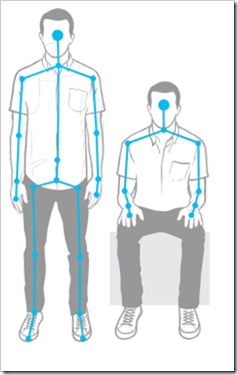
\includegraphics[]{kinect/fig/microsoft-skeleton.png}
    \caption{Σκελετικό σύστημα της \eng{Microsoft}}
    \label{fig:microsoft-sdk-skeleton}
\end{figure}

%%%%%%%%%%%%%%%%%%%%%%%%%%%%%%%%%%%%%%%%%%%%%%%%%%%%%%%%%%%%%%%%%%%%%%%%%%%%%%%%
\subsection{Εναλλακτικά Εργαλεία}

Το εναλλακτικό εργαλείο είναι το OpenNI. Εκτός από το \eng{Kinect} δίνει την δυνατότητα πρόσβασης και σε άλλους αισθητήρες με τον ίδιο τρόπο και έχει μια πολύ ξεκάθαρη αρχιτεκτονική, που διευκολύνει τον προγραμματιστή όπως φαίνεται στην εικόνα \ref{fig:openni-framework}. Όπως και με το \eng{SDK} της \eng{Microsoft} η \eng{OpenNI} σου παρέχει πλούσιο ρεπερτόριο από αλγορίθμους και εφαρμογές. Είναι ανοιχτού κώδικα, υπάρχει υλοποίηση όσο στα \eng{Windows} έτσι και στο \eng{Linux} (\eng{cross platform}). Οι κύριες γλώσσες προγραμματισμού  που υποστηρίζονται από το \eng{OpenNI} είναι η \eng{C++}, η \eng{Java} και \eng{Python}.

\begin{figure}[H]
    \centering
    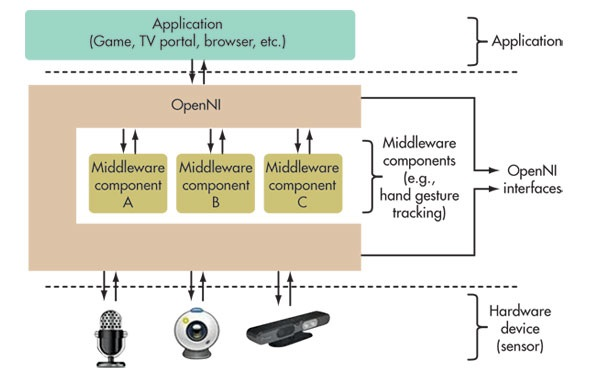
\includegraphics[width=.8\textwidth]{kinect/fig/openni-framework.jpg}
    \caption{Αρχιτεκτονική του \eng{OpenNI}}
    \label{fig:openni-framework}
\end{figure}

\begin{figure}[H]
    \centering
    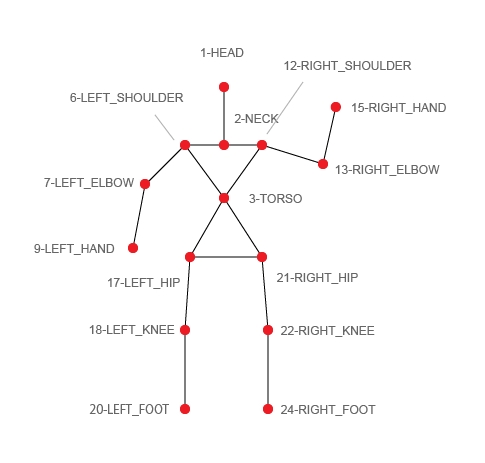
\includegraphics[width=.5\textwidth]{kinect/fig/openni-skeleton.png}
    \caption{Σκελετικό σύστημα του \eng{OpenNI}}
    \label{fig:openni-skeleton}
\end{figure}

Όσον αφορά την εξαγωγή του σκελετού, μειονεκτεί σε σύγκριση με τον αντίστοιχο εργαλείο της \eng{Microsoft}. Αυτό γιατί σου παρέχει 16 αρθρώσεις όπως φαίνεται στην εικόνα \ref{fig:openni-skeleton}, που ίσως δεν είναι αρκετά για την εφαρμογή, ειδάλλως δεν είναι και τόσο κρίσιμη διαφορά. Ένα βασικό μειονέκτημα όμως είναι η απαίτηση βαθμονόμησης της συσκευής. Επίσης κάτι σημαντικό είναι το κομμάτι που αφορά την βελτίωση των μετρήσεων και το \eng{OpenNI} δεν σου παρέχει έτοιμες δομές, κάτι που θα χρειασθεί χρόνο για να υλοποιηθεί. Για τους παραπάνω λόγους προτιμήθηκε το εργαλείο της \eng{Microsoft}. Ενδεικτικά στον πίνακα \ref{tab:openni-microsoft} φαίνονται κάποιες βασικές διαφορές.

\begin{center}
    \begin{tabular}{lcc}
        \toprule
        % after \\: \hline or \cline{col1-col2} \cline{col3-col4} ...
        \multicolumn{1}{c}{Χαρακτηριστικά} & \eng{OpenNI} & \eng{Microsoft SDK} \\
        \midrule
        Πρόσβαση στα δεδομένα βάθους και \eng{RGB} & Ναι & Ναι \\
        Ανίχνευση αρθρώσεων & Ναι & Ναι \\
        Υποστήριξη αναγνώρισης χειρονομιών & Ναι & Όχι \\
        Συναρτήσεις άμεσης αποθήκευσης δεδομένων στο δίσκο & Ναι & Όχι \\
        Βαθμονόμιση & Ναι & Όχι \\
        Υποστήριξη επεξεργασίας ήχου και αναγνώριση ομιλίας & Όχι & Ναι \\
        Ευκολία εγκατάστασης & Όχι & Ναι \\
        Διαθέσιμος αριθμός αρθρώσεων & 16 & 20 \\
        Ποιότητα εγχειριδίων τεκμηρίωση  & Καλή & Μέτρια\\
        \bottomrule
    \end{tabular}
    \captionof{table}{Σύγκριση εναλλακτικών εργαλείων}
    \label{tab:openni-microsoft}
\end{center}

%%%%%%%%%%%%%%%%%%%%%%%%%%%%%%%%%%%%%%%%%%%%%%%%%%%%%%%%%%%%%%%%%%%%%%%%%%%%%%%%
\section{Σύστημα Μετρήσεων}

Οι συλλογή ορθών μετρήσεων είναι ένα σημαντικό βήμα για την εξαγωγή σωστών αποτελεσμάτων στα μετέπειτα στάδια. Η καταγραφή της βάδισης του ανθρώπου είναι η βάση για πολλές αναλύσεις, όπου μπορούν να εξαχθούν χρήσιμα αποτελέσματα. Ενδεικτικά θα ήταν χρήσιμη η μελέτη της δυναμικής συμπεριφοράς του σώματος κατά την διεξαγωγή μιας κίνησης με αποτέλεσμα να μπορεί κανείς να μελετήσει την συμπεριφορά του μυοσκελετικού συστήματος. Πρέπει να δοθεί μεγάλη βαρύτητα στην απόκτηση έγκυρων μετρήσεων, για το λόγο αυτό πρέπει να δημιουργηθούν αλγόριθμοι που να ελαχιστοποιούν τα σφάλματα και να διώχνουν τον θόρυβο. Στην συνέχεια θα εξηγηθούν κάποια ενδεικτικά προβλήματα κατά την διαδικασία της καταγραφής και η αντιμετώπιση τους.

%%%%%%%%%%%%%%%%%%%%%%%%%%%%%%%%%%%%%%%%%%%%%%%%%%%%%%%%%%%%%%%%%%%%%%%%%%%%%%%%
\subsection{Τροχιές των Αρθρώσεων}

Ο προγραμματιστής  μπορεί έχει πρόσβαση στα δεδομένα της συσκευής που αφορούν την συντεταγμένη των αρθρώσεων. Δεδομένου ότι έχει ενεργοποιηθεί εσωτερικά (από τον πρόγραμμα) η ανίχνευση του σκελετού και στο πεδίο ορατότητας της συσκευής ανιχνευθεί αντικείμενο ανθρώπινης μορφής, τότε η συσκευή στέλνει πακέτα με την πληροφορία των θέσεων των αρθρώσεων πίσω στον χρήστη. Το πακέτο περιέχει και επιπλέον πληροφορίες για τις αρθρώσεις όπως είναι ο προσανατολισμός (προϋποθέτει ιεραρχική δομή σκελετού), σκορ εμπιστοσύνης για την μέτρηση (που κυμαίνεται από 0 έως 1) και κάποιες ενδείξεις αν έχει εξαχθεί συμπέρασμα για την θέση της άρθρωσης. Στην ανάλυση ενδιαφερόμαστε για την θέση όσο εξελίσσεται ο χρόνος. Έστω ότι έχουμε $Ν$ αριθμό αρθρώσεων που αποθηκεύονται σε συγκεκριμένες χρονικές στιγμές.

\begin{equation}
    p^{t}_{j} = \{x^{t}_{j}, y^{t}_{j}, z^{t}_{j}\}, \quad t \in (0, t), \quad j \in (0, N)
    \label{equ:trajectories}
\end{equation}

Όπου \eng{p} είναι η Καρτεσιανή θέση την χρονική στιγμή \eng{t} για την άρθρωση \eng{j}. Η αρχή των αξόνων είναι η θέση του \eng{Kinect} και ο άξονας \eng{Z} είναι το βάθος όπως φαίνεται στην εικόνα \ref{fig:kinect-joints}.

\begin{figure}[H]
    \centering
    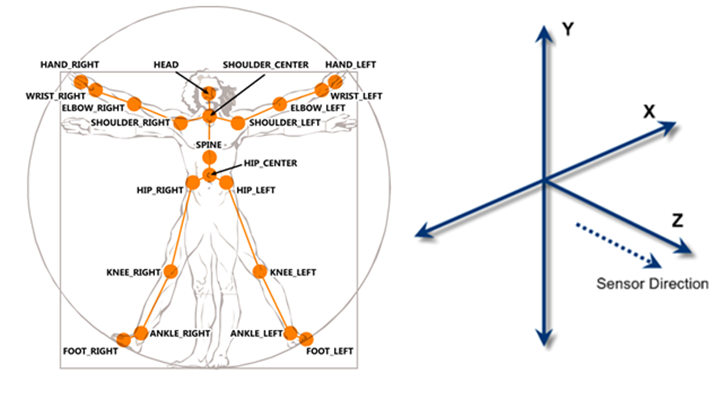
\includegraphics[width=.8\textwidth]{kinect/fig/kinect-joints.png}
    \caption{Σύστημα αρθρώσεων}
    \label{fig:kinect-joints}
\end{figure}

Πρέπει να διευκρινιστεί ότι τα δεδομένα δεν έρχονται περιοδικά σε ντετερμινιστικές χρονικές στιγμές αλλά έχουν μια απόκλιση που οφείλεται κυρίως στο \eng{software} και στις εσωτερικές καθυστερήσεις. Για το λόγο αυτό είναι χρήσιμο να γίνει η μέτρηση της χρονικής στιγμής που έρχονται και αποθηκεύονται τα δεδομένα και να χρησιμοποιηθεί στα μετέπειτα στάδια της ανάλυσης. Μια άλλη παρατήρηση είναι ότι τα δεδομένα είναι στο σύστημα συντεταγμένων με αρχή των αξόνων το \eng{Kinect} και ανάλογα το εργαλείο που θα χρησιμοποιηθεί στα μετέπειτα στάδια της επεξεργασία θα πρέπει να γίνει η κατάλληλη μετατροπή συστήματος συντεταγμένων.

%%%%%%%%%%%%%%%%%%%%%%%%%%%%%%%%%%%%%%%%%%%%%%%%%%%%%%%%%%%%%%%%%%%%%%%%%%%%%%%%
\subsection{Αντιμετώπιση του Θορύβου}

Υπάρχουν πολλά ενοχλητικά προβλήματα που εμφανίζονται στην πράξη και καθιστούν τις μετρήσεις \lq μην κατάλληλες για επεξεργασία\rq . Ο θόρυβος επηρεάζεται από πολλούς παράγοντες, όπως είναι ο φωτισμός στον χώρο που εκτελείται το πείραμα, η στάση του σώματος, η τοποθεσία της συσκευής και πολλά άλλα. Ένα πολύ εμφανές παράδειγμα θορύβου που εμφανίζεται κατά την εκτίμηση της θέσης της άρθρωσης λόγο της μικρής απόκλιση της τιμής από την προηγούμενη μέτρηση με αποτέλεσμα να σου δίνει την αίσθηση ότι το δείγμα τρέμει ενώ στην πραγματικότητα είναι στάσιμο όπως φαίνεται και στην εικόνα \ref{fig:hand2}.

\begin{figure}[h]
    \centering
    \begin{subfigure}[b]{.3\textwidth}
        
\includegraphics[width=\textwidth]{kinect/fig/hand1.png}
        \caption{Ακριβή εκτίμηση}
        \label{fig:hand1}
    \end{subfigure} ~
    \begin{subfigure}[b]{.3\textwidth}
        
\includegraphics[width=\textwidth]{kinect/fig/hand2.png}
        \caption{Εκτίμηση λόγο θορύβου}
        \label{fig:hand2}
    \end{subfigure}
    \caption{Πρόβλημα εκτίμησης θέσης λόγο θορύβου}
\end{figure}

Για την αντιμετώπιση του προβλήματος μπορούν να υλοποιηθούν απλές τεχνικές φιλτραρίσματος και να ελαχιστοποιηθεί ο θόρυβος. Πρέπει κανείς να ξεχωρίσει κάποια κριτήρια που είναι το ποσοστό της εξομάλυνσης των πολύ απότομων κινήσεων, την καθυστέρηση που εισάγεται από την αλλαγή που προκαλεί η φάση του φίλτρου και το αν η εφαρμογή είναι πραγματικού χρόνου (\eng{online}) ή μην πραγματικού χρόνου (\eng{offline}).

Αν επιλεχθεί να αποκοπούν οι ψηλές συχνότητες (απότομες κινήσεις) τότε θα αντιμετωπιστεί το πρόβλημα που αναφέρθηκε πιο πάνω και το αποτέλεσμα θα είναι αυτό της εικόνας \ref{fig:hand1}. Ο θόρυβος αυτής της μορφής στην ξένη βιβλιογραφία αναφέρεται σαν \lq \eng{jitter} \rq . Πρέπει να προσέξουμε όμως γιατί το σύστημα θα αγνοεί πέραν του θορύβου και τις απότομες κινήσεις του δείγματος που ίσως είναι κάτι ανεπιθύμητο. Η σωστή επιλογή αυτών των παραμέτρων είναι κρίσιμη και εξαρτάται από την εφαρμογή που μας ενδιαφέρει και κυρίως από την ταχύτητα του δείγματος.

Όπως φαίνεται στην εικόνα \ref{fig:filter-latency} με κόκκινο είναι η τροχιά, όπου βλέπουμε τις ανεπιθύμητες μεταβολές λόγο θορύβου. Από την άλλη με μπλε χρώμα είναι η τροχιά μετά το φιλτράρισμα, όπου παρατηρούμε ότι έχει εξομαλυνθεί ο θόρυβος, αλλά έχει δημιουργηθεί καθυστέρηση των δειγμάτων. Κάτι που αξίζει να σημειωθεί είναι ότι αν η εφαρμογή δεν απαιτείται να είναι πραγματικού χρόνου, τότε μπορούν να χρησιμοποιηθούν μην αιτιατά φίλτρα, που λαμβάνουν υπόψη στους υπολογισμούς τους μελλοντικές τιμές με αποτέλεσμα να γίνει καλύτερη εκτίμηση της τροχιάς.

\begin{figure}[h]
    \centering
    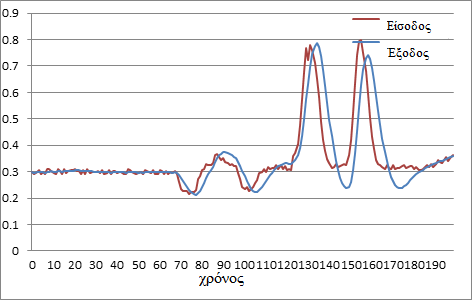
\includegraphics[width=.8\textwidth]{kinect/fig/filter-latency.png}
    \caption{Εξομάλυνση και καθυστέρηση ακολουθίας μετά το φιλτράρισμα}
    \label{fig:filter-latency}
\end{figure}

Για παράδειγμα μια απλή τεχνική για την αφαίρεση του θορύβου λόγο \eng{jitter} βασίζεται στην απλή σχέση αναδρομής \ref{equ:jitter-removal}.

\begin{equation}
    \hat{p}_{n} =
    \begin{cases}
        p_{n}, & \text{Αν } \|p_{n} - \hat{p}_{n-1}\| < \text{κατώφλι} \\
        a \cdot p_{n} + (1-a) \cdot \hat{p}_{n-1}, & \text{αλλιώς}
    \end{cases}
    \label{equ:jitter-removal}
\end{equation}

Στην παρούσα εργασία χρησιμοποιείται μια παραλλαγή του φίλτρου \cite{filter12} \lq \eng{Holt Double Exponential Smoothing}\rq , που έχει άμεση εφαρμογή στα οικονομικά. Τα φίλτρα αυτά στηρίζονται στην παρακάτω αναδρομική σχέση \ref{equ:double-exponential} και οι παράμετροι που επηρεάζουν το αποτέλεσμα δίνονται στο πίνακα \ref{tab:filter-parameters}.

\begin{equation}
    \begin{aligned}
        b_{n} = \gamma \cdot (\hat{p}_{n} - \hat{p}_{n-1}) + (1 - \gamma) \cdot b_{n-1}\\[10pt]
        \hat{p}_{n} = \alpha \cdot p_{n} + (1 - a) \cdot (\hat{p}_{n-1} + b_{n-1})
    \end{aligned}
    \label{equ:double-exponential}
\end{equation}

\vspace{10pt}

\begin{center}
    \begin{threeparttable}
        \begin{tabular}{lccc}
            \toprule
            % after \\: \hline or \cline{col1-col2} \cline{col3-col4} ...
            Παράμετροι & Κανονικό\tnote{α} & Μέτριο\tnote{β} & Δυνατό\tnote{γ} \\
            \midrule
            \eng{Smoothing} & 0.5 & 0.5 & 0.7 \\
            \eng{Correction} & 0.5 & 0.1 & 0.3 \\
            \eng{Prediction} & 0.5 & 0.5 & 1.0 \\
            \eng{JitterRadius} & 0.05 & 0.1 & 1.0 \\
            \eng{MaxDeviationRadius} & 0.04 & 0.1 & 1.0 \\
            \bottomrule
        \end{tabular}
        \begin{tablenotes}
            \item[α] Φιλτράρει ελαφρώς το \eng{jitter}. Καλό για εφαρμογές αναγνώρισης σε παιχνίδια, όπου υπάρχουν απότομες κινήσεις.
            \item[β] Μειώνει αρκετά το \eng{jitter}. Είναι καλό για εφαρμογές όπου απαιτείται ομαλή κίνηση.
            \item[γ] Μειώνει πολύ το \eng{jitter}. Αφορά εφαρμογές που δεν ενδιαφερόμαστε για την καθυστέρηση της κίνησης.
        \end{tablenotes}
    \end{threeparttable}
    \captionof{table}{Ενδεικτικές παράμετρος του φίλτρου}
    \label{tab:filter-parameters}
\end{center}

%\begin{itemize}
%	\item \eng{Smoothing} παράμετρος εξομάλυνσης
%	\item \eng{Correction} μικρές τιμές τείνουν να μοιάζουν με τα δεδομένα που έχουμε
%	\item \eng{Prediction} συμβολίζει την εκτίμηση που κάνουμε για μελλοντικές τιμές
%	\item \eng{JitterRadius} η ακτίνα σε μέτρα για την μείωση του \eng{jitter}
%    \item \eng{MaxDeviationRadius} η μέγιστη διασπορά στην ακτίνα την οποία μπορεί να ανεχτεί το φίλτρο
%\end{itemize}

%%%%%%%%%%%%%%%%%%%%%%%%%%%%%%%%%%%%%%%%%%%%%%%%%%%%%%%%%%%%%%%%%%%%%%%%%%%%%%%%
\section{Υλοποίηση}

Το πρόγραμμα καταγραφής που υλοποιήθηκε έχει σαν στόχο την καταγραφή της χρονικής μεταβολής των θέσεων των αρθρώσεων και την βελτίωση των μετρήσεων. Για να ελαχιστοποιηθούν οι καθυστερήσεις και να μην ελαττωθεί ο ρυθμός επεξεργασίας των πακέτων που εισέρχονται από το \eng{Kinect}, έχουν ενεργοποιηθεί μόνο οι δυνατότητες παρακολούθησης του σκελετού και την πρόσληψη έγχρωμου βίντεο για να μπορούμε να αντιλαμβανόμαστε το ορατό πεδίο του αισθητήρα όπως φαίνεται στην εικόνα \ref{fig:motion-capture}.

\begin{figure}[H]
    \centering
    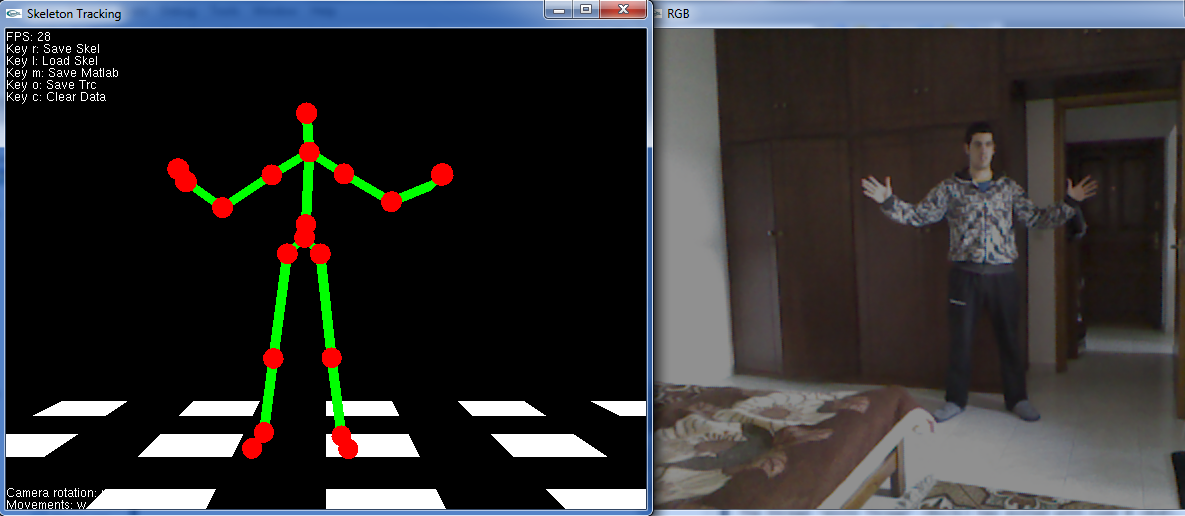
\includegraphics[width=.9\textwidth]{kinect/fig/motion-capture.png}
    \caption{Σύστημα καταγραφής}
    \label{fig:motion-capture}
\end{figure}

Πρέπει να σημειωθεί ότι η υλοποίηση έγινε με χρήση την βιβλιοθήκη \eng{OpenGL}. Υπάρχουν δύο παράθυρα, όπου στο ένα αναπαριστάται η τελευταία ακολουθία θέσεων του σκελετού, ενώ στο άλλο γίνεται αποτύπωση της έγχρωμης εικόνας που λαμβάνουμε ανά τακτικά χρονικά διαστήματα σαν εικόνα υφής με αποτέλεσμα να έχουμε μια ανανέωση του περιεχομένου (δηλαδή βίντεο). Η περιήγηση στο τρισδιάστατο χώρο του αριστερού παραθύρου μπορεί να γίνει με την βοήθεια του ποντικιού και του πληκτρολογίου δίνοντας την δυνατότητα αναπαράστασης του μοντέλου από διαφορετικές οπτικές γωνίες. 

Εσωτερικά αποθηκεύονται οι παρελθοντικές τιμές των θέσεων σε ειδικές δομές μαζί με όλη την πληροφορία που διαθέτει το \eng{Kinect}. Παρέχεται η δυνατότητα αποθήκευσης των δεδομένων σε δυαδική μορφή η οποία είναι εύκολη στην ανάγνωση και δεν απαιτεί υλοποίηση πολύπλοκων συναρτήσεων ανάγνωσης. Επίσης υπάρχουν επιλογές για αποθήκευσης των τροχιών σε μορφή \lq \eng{.dat}\rq  της \eng{Matlab} και σε μορφή \lq \eng{.trc}\rq , που είναι συμβατή με το εργαλείο \eng{OpenSim}.


%%%%%%%%%%%%%%%%%%%%%%%%%%%%%%%%%%%%%%%%%%%%%%%%%%%%%%%%%%%%%%%%%%%%%%%%%%%%%%%%
\chapter{Περιγραφή Στερεών Σωμάτων}

Στο κεφάλαιο αυτό γίνεται μια σύντομη περιγραφή της μαθηματικής διατύπωσης του προβλήματος της κινηματικής και της δυναμικής των στερεών σωμάτων. Αρχικά μελετούνται οι σχετικοί μετασχηματισμοί που είναι το βασικό εργαλείο περιγραφής της θέσης και του προσανατολισμού των σωμάτων. Έπειτα, γίνεται μια σύντομη περιγραφή της κινηματικής και της διάδοσης των ταχυτήτων σε μια αλυσίδα. Τέλος, επεκτείνεται η ανάλυση στο πρόβλημα της δυναμικής και προτείνεται ένας τρόπος επίλυσης του προβλήματος\footnote{Για περισσότερες πληροφορίες σχετικά με την μοντελοποίηση και την τυποποίηση των εξισώσεων ο αναγνώστης μπορεί να καταφύγει στο \cite{craig95}.}.

%%%%%%%%%%%%%%%%%%%%%%%%%%%%%%%%%%%%%%%%%%%%%%%%%%%%%%%%%%%%%%%%%%%%%%%%%%%%%%%%
\section{Μετασχηματισμοί}

Η θέση και ο προσανατολισμός ενός στερεού σώματος στο χώρο αναφορικά με ένα αδρανειακό καρτεσιανό πλαίσιο συντεταγμένων $\{Β\}$ γίνεται με την περιγραφή της θέσης και του προσανατολισμού ενός καρτεσιανού πλαισίου $\{Α\}$, το οποίο στερεώνουμε σε ένα αυθαίρετο σημείο του σώματος, π.χ. στο κέντρο μάζας. Το διάνυσμα θέσης του πλαισίου $\{Β\}$ εκφρασμένο στο αδρανειακό πλαίσιο $\{Α\}$ με $^AP_{BORG}$ και περιγράφει την θέση του στερεού σώματος και ο πίνακας $^AR_B$ περιγράφει τον προσανατολισμό του σε σχέση με το αδρανειακό σύστημα. Το ζεύγος $\{^AP_{BORG}, ^AR_B\}$ περιγράφουν πλήρες την διάταξη του στερεού σε σχέση με το αδρανειακό \ref{fig:transformation}. Έτσι μπορεί κανείς να εκφράσει την σχετική θέση ενός σημείου στο πλαίσιο $\{Β\}$ ως προς το πλαίσιο  $\{Α\}$ ως εξής:

\begin{equation}
    ^AP = ^AT_B \cdot ^BP, \quad
    ^AT_B =
    \begin{bmatrix}
        ^AR_B & ^AP_{BORG}\\
        0 & 1
    \end{bmatrix}
\end{equation}

\begin{figure}[H]
    \centering
    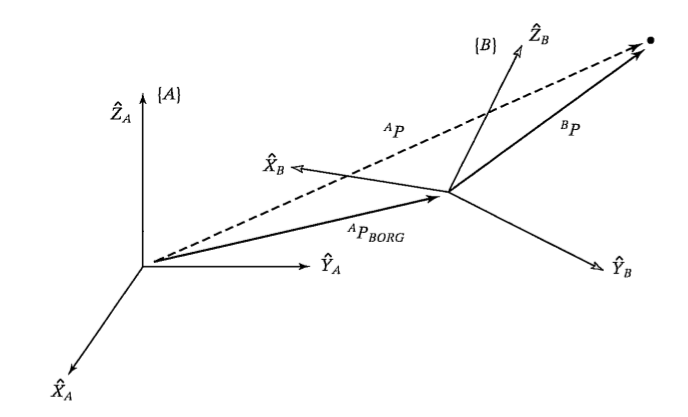
\includegraphics[width=.7\textwidth]{rigidbody/fig/transofrmation.png}
    \caption{Σχετικός μετασχηματισμός}
    \label{fig:transformation}
\end{figure}

Στις περιπτώσεις όπου έχουμε αλυσίδες από πλαίσια που ενώνονται με τους αντίστοιχους σχετικούς μετασχηματισμούς μπορούμε να εκφράσουμε την σχετική θέση ενός πλαισίου πολλαπλασιάζοντας του αντίστοιχους μετασχηματισμούς. Όπως φαίνεται και στην εικόνα \ref{fig:transformation-chain} μπορεί να υπάρχουν εναλλακτικές διαδρομές που περιγράφουν την θέση ενός πλαισίου και οι μετασχηματισμοί που ισχύουν μπορούν να περιγραφούν από τις εξισώσεις \ref{equ:chain}. Σε περίπτωση που υπάρχει κάποιος άγνωστος μετασχηματισμός μπορεί κανείς να λύσει ως προς τον άγνωστο δοσμένου ότι γνωρίζει τους υπόλοιπους.

\begin{figure}[H]
    \centering
    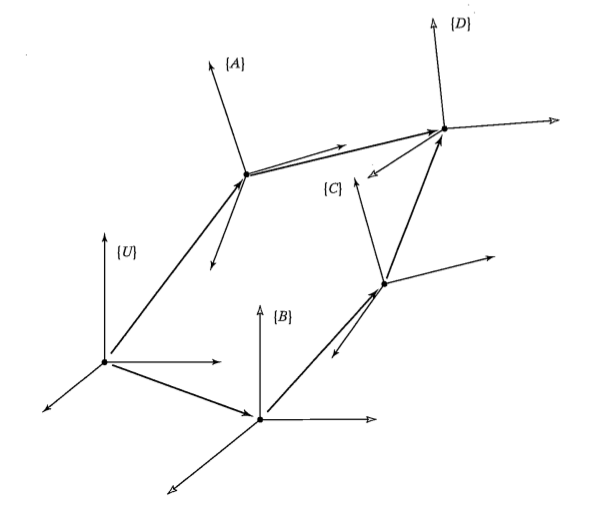
\includegraphics[width=.7\textwidth]{rigidbody/fig/transformation-chain.png}
    \caption{Αλυσίδες μετασχηματισμού}
    \label{fig:transformation-chain}
\end{figure}

\begin{equation}
    \begin{aligned}
        ^UT_D = {}^UT_A \cdot {}^AT_D\\[10pt]
        ^UT_D = {}^UT_B \cdot {}^BT_C \cdot {}^CT_D\\[10pt]
        ^UT_A \cdot ^AT_D = {}^UT_B \cdot {}^BT_C \cdot {}^CT_D
    \end{aligned}
    \label{equ:chain}
\end{equation}

%%%%%%%%%%%%%%%%%%%%%%%%%%%%%%%%%%%%%%%%%%%%%%%%%%%%%%%%%%%%%%%%%%%%%%%%%%%%%%%%
\section{Κινηματική}

Για να κατανοήσουμε το πρόβλημα της κινηματικής, αλλά και της δυναμικής πρέπει να ξεκαθαρίσει τη αλληλεπίδραση των ταχυτήτων σε ένα σύστημα στερεών σωμάτων. Για το λόγο αυτό πριν προχωρήσουμε στην ανάλυση θα γίνει μια μικρή εισαγωγή στο πώς απορρέουν οι εξισώσεις που περιγράφουν την ταχύτητα ενός στερεού με χρήση των σχετικών μετασχηματισμών. Στην συνέχει θα γενικεύσουμε σε συστήματα σωμάτων.

%%%%%%%%%%%%%%%%%%%%%%%%%%%%%%%%%%%%%%%%%%%%%%%%%%%%%%%%%%%%%%%%%%%%%%%%%%%%%%%%
\subsection{Μελέτη της Ταχύτητας}

Έστω ότι θέλουμε να μελετήσουμε την κίνηση ενός σημείου $^BQ$ που ανήκει σε ένα στέρεο σώμα. Στην πιο γενική περίπτωση το σημείο θα έχει μια γραμμική ταχύτητα ως προς κάποιο πλαίσιο $\{Β\}$. Το πλαίσιο $\{Β\}$ θα έχει και αυτό γραμμική και περιστροφική ταχύτητα ως προς κάποιο πλαίσιο παρατήρησης, έστω $\{Α\}$. Θα θέλαμε να εκφράσουμε την ταχύτητα που έχει το σημείο $Q$ ως προς το πλαίσιο παρατήρησης όπως φαίνεται στην εικόνα \ref{fig:velocity}.

\begin{figure}[H]
    \centering
    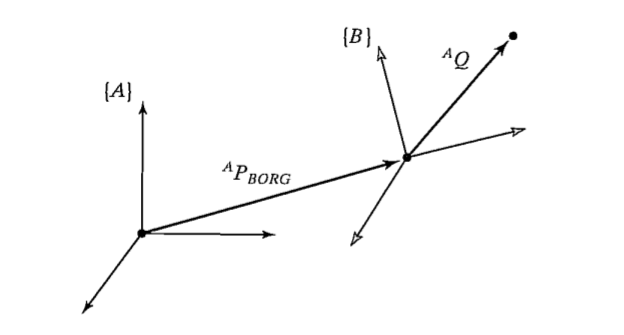
\includegraphics[width=.8\textwidth]{rigidbody/fig/velocity.png}
    \caption{Γενική περίπτωση κίνησης ενός σημείου}
    \label{fig:velocity}
\end{figure}

Έστω ότι η γραμμική ταχύτητα του πλαισίου $\{Β\}$ σε σχέση με το $\{Α\}$ είναι $^AV_{BORG}$ και η γωνιακή ταχύτητα είναι $^A\Omega_{BORG}$. Η γωνιακή ταχύτητα είναι ένα διάνυσμα, όπου η διεύθυνση εκφράζει τον άξονα περιστροφής, ενώ το μέτρο του την γωνία. Επίσης το σημείο $Q$ κινείται με ταχύτητα $^BV_Q$. Η γενική εξίσωση που περιγράφει την κίνηση του σημείου $Q$ δίνεται από την εξίσωση \ref{equ:q-velocity}.

\begin{equation}
    ^AV_Q = {}^AV_{BORG} + {}^AR_B \cdot {}^BV_Q + {}^A\Omega_B \times {}^AR_B
    \cdot {}^BQ
    \label{equ:q-velocity}
\end{equation}

Έστω ότι το σημείο $Q$ είναι αδρανειακό ως προς το πλαίσιο $\{Β\}$. Αν υποθέσουμε ότι το πλαίσιο παρατήρησης $\{Α\}$ συμπίπτει με το πλαίσιο $\{Β\}$, τότε η θέση του σημείο $Q$ ως προς το $\{Α\}$ δίνεται από την εξίσωση \ref{equ:position}.

\begin{equation}
    ^AQ = {}^AR_B \cdot {}^BQ
    \label{equ:position}
\end{equation}

Αν παραγωγίσουμε την σχέση \ref{equ:position} θα πάρουμε την ταχύτητα του σημείου ως προς το $\{Α\}$.

\begin{equation}
    \begin{split}
        ^A\dot{Q} & = {}^A\dot{R}_B \cdot {}^BQ\\
        ^AV_Q & = {}^A\dot{R}_B \cdot {}^AR^{-1}_B \cdot {}^AQ\\
        ^AV_Q & = {}^AS_B \cdot {}^AQ
    \end{split}
    \label{equ:velocity}
\end{equation}

Όπου $^AS_B$ είναι ο αντισυμμετρικός πίνακας και εκφράζεται ως εξής:

\begin{equation}
    ^AS_B  =
    \begin{bmatrix}
        0 & -\Omega_z & \Omega_y\\
        \Omega_z & 0 & -\Omega_x\\
        -\Omega_y & \Omega_x & 0
    \end{bmatrix}
    \label{equ:skew-symmetric}
\end{equation}

%%%%%%%%%%%%%%%%%%%%%%%%%%%%%%%%%%%%%%%%%%%%%%%%%%%%%%%%%%%%%%%%%%%%%%%%%%%%%%%%
\subsection{Μετάδοση της Ταχύτητας}

Ας δούμε το πρόβλημα της μετάδοσης της ταχύτητας από άρθρωση σε άρθρωση όπως φαίνεται στην εικόνα \ref{fig:velocity-transfer}. Θα μελετήσουμε αρχικά την επιρροή της γωνιακής ταχύτητας για την άρθρωση $i+1$ και έπειτα της γραμμικής ταχύτητας. Θα επικεντρωθούμε μόνε σε αρθρώσεις που περιστρέφονται γύρω από τυχαίο άξονα $Ζ$. Η γωνιακή ταχύτητα δίνεται από την σχέση \ref{equ:angular-velocity-propagation}.

\begin{equation}
    ^i\omega_{i+1} = {}^i\omega_i + {}^iR_{i+1} \cdot \dot{q}_{i+1}
    \cdot {}^{i+1}\hat{Z}_{i+1}
    \label{equ:angular-velocity-propagation}
\end{equation}

Αν πολλαπλασιάσουμε την εξίσωση \ref{equ:angular-velocity-propagation} από τις δύο μεριές με $^{i+1}R_i$ μπορούμε να εκφράσουμε το αποτέλεσμα στο πλαίσιο $\{i+1\}$ θα εξάγουμε την εξίσωση \ref{equ:angular-velocity-propagation-final}.

\begin{equation}
    ^{i+1}\omega_{i+1} = {}^{i+1}R_i \cdot {}^i\omega_i + \dot{q}_{i+1}
    \cdot {}^{i+1}\hat{Z}_{i+1}
    \label{equ:angular-velocity-propagation-final}
\end{equation}

Όσον αφορά την γραμμική ταχύτητα η σχέση δίνεται από την εξίσωση \ref{equ:velocity-propagation}.

\begin{equation}
    ^iu_{i+1} = {}^iu_i + {}^i\omega_i \times {}^iP_{i+1}
    \label{equ:velocity-propagation}
\end{equation}

Αν πολλαπλασιάσουμε ξανά την εξίσωση \ref{equ:velocity-propagation} με $^{i+1}R_i$ θα έχουμε την σχέση \ref{equ:velocity-propagation-final}.

\begin{equation}
    ^{i+1}u_{i+1} = {}^{i+1}R_i \cdot (^iu_i + {}^i\omega_i \times
    {}^iP_{i+1})
    \label{equ:velocity-propagation-final}
\end{equation}

\begin{figure}[H]
    \centering
    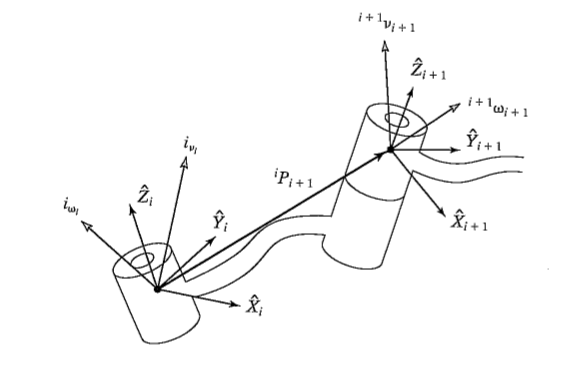
\includegraphics[width=.8\textwidth]{rigidbody/fig/velocity-transfer.png}
    \caption{Μετάδοση της ταχύτητας από άρθρωση σε άρθρωση}
    \label{fig:velocity-transfer}
\end{figure}

%%%%%%%%%%%%%%%%%%%%%%%%%%%%%%%%%%%%%%%%%%%%%%%%%%%%%%%%%%%%%%%%%%%%%%%%%%%%%%%%
\subsection{Αντίστροφη Κινηματική}

Η αντίστροφη κινηματική είναι ένα σημαντικό εργαλείο στα στάδια την διεξαγωγής του πειράματος. Με λίγα λόγια είναι η διαδικασία που μετατρέπει τις θέσεις των αρθρώσεων στο καρτεσιανό τρισδιάστατο χώρο σε γενικευμένες συντεταγμένες του μοντέλου (γωνίες), έτσι ώστε κάθε χρονική στιγμή το μοντέλο να είναι στην ίδια διάταξη με τις μετρήσιμες θέσεις των αντίστοιχων αρθρώσεων. Παρακάτω θα δοθεί η μαθηματική διατύπωση για την λύση του προβλήματος και θα επισημανθούν κάποια λεπτά σημεία που ίσως οδηγήσουν σε λάθος αποτελέσματα.

Δοθέντος ενός συστήματος σωμάτων με $Ν$ βαθμών ελευθερίας με γενικευμένη συντεταγμένη $q^{t}_{j}$ και δοσμένη χρονική ακολουθία από θέσεις για κάθε άρθρωση του μοντέλου $p^{t}_{j}$ με $j \in (1 N)$. Το πρόβλημα της εύρεσης των γενικευμένων συντεταγμένων για κάθε άρθρωση ώστε να ελαχιστοποιηθεί το σφάλμα της απόστασης μεταξύ της παρατήρησης και της στάσης του μοντέλου μπορεί να μοντελοποιηθεί σαν πρόβλημα βελτιστοποίησης \cite{sherman13}. Στόχος είναι η ελαχιστοποίηση του σφάλματος, όπου το σφάλμα είναι η αθροιστική συνάρτηση απόστασης μεταξύ μοντέλου και τις θέσεις των θέσεων. Σαν συνάρτηση απόστασης μπορεί να επιλεγεί η Ευκλείδεια νόρμα $2^{ης}$ τάξης. Επίσης κατά την επίλυση θα πρέπει να ληφθούν υπόψη και οι φυσικοί περιορισμοί της διάταξης για κάθε άρθρωση.

\begin{equation}
    \begin{aligned}
        & \underset{q_{j}}{\text{\eng{minimize}}} 
        & & \sum_{i=1}^{N} w_{j} \cdot \norm{p_{j} - p(q_{j})}^{2} \\
        & \text{\eng{s.t.}}
        & & c_{j}(q_{j}) \leq b_{j}, \; i = 1, \ldots, N.
    \end{aligned}
    \label{equ:ik-optimization}
\end{equation}

Όπως φαίνεται στις εξισώσεις \ref{equ:ik-optimization} οι $c_{j}(q_{j}) \leq b_{j}$ είναι οι περιορισμοί των αρθρώσεων. Που σημαίνει ότι η λύση των \eng{q's} θα πρέπει να την ικανοποιούν. Το $w_{j}$ είναι ο συντελεστής βαρύτητας για την συγκεκριμένη άρθρωση και καθορίζει πόσο σημαντική είναι στον υπολογισμό του σφάλματος.

Προβλήματα που μπορούν να εμφανιστούν κατά την διαδικασία είναι η πολλαπλή λύση όπως φαίνεται στην εικόνα \ref{fig:ik-multiple-solutions}. Αυτό οφείλεται στο αριθμό των βαθμών ελευθερίας, που αν είναι πολλοί τότε δίνουν ευελιξία στην διάταξη. Τρόποι που μπορούν να βελτιώσουν το αποτέλεσμα είναι η ελαχιστοποίηση των βαθμών ελευθερίας της διάταξης ή να εισαχθούν κατάλληλοι περιορισμοί. Για παράδειγμα σε αρθρώσεις που έχουν τρεις βαθμούς ελευθερίας, όπως είναι ο γοφός, υπάρχει μεγάλη ευελιξία με αποτέλεσμα να δίνει πολλαπλές λύσεις και να μην προσανατολίζει σωστά το τμήμα του μηρού.

\begin{figure}[H]
    \centering
    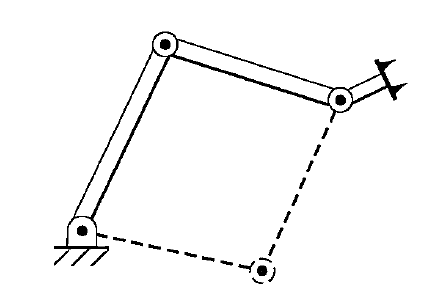
\includegraphics[width=.8\textwidth]{rigidbody/fig/ik-multiple-solutions.png}
    \caption{Πολλαπλότητα λύσεων}
    \label{fig:ik-multiple-solutions}
\end{figure}

Ένα σημαντικό πρόβλημα που έχει να κάνει με τις δυνατότητες του συγκεκριμένου συστήματος καταγραφής είναι ότι το η πληροφορία που σου παρέχει μπορεί να μην αρκεί για να περιγράψει σωστά την διάταξη. Δηλαδή, αν υποθέσουμε ότι έχουμε μια άρθρωση με έξι βαθμούς ελευθερίας (τρεις περιστροφές και τρεις μετατοπίσεις) τότε για να επιλυθεί το σύστημα απαιτούνται τουλάχιστον τρία σημεία πάνω στο τμήμα, που να μην είναι συγγραμμικά μεταξύ τους. Για αυτό το λόγο τα καλά συστήματα όπως είναι το \eng{Vicon} καταγράφουν πολλαπλές θέσεις σε κάθε τμήμα του σώματος.
 
%%%%%%%%%%%%%%%%%%%%%%%%%%%%%%%%%%%%%%%%%%%%%%%%%%%%%%%%%%%%%%%%%%%%%%%%%%%%%%%%
\section{Δυναμική}

Αφού έχει γίνει η ανάλυση της κινηματικής μπορεί κανείς να κάνει ένα βήμα πιο πέρα και να εξάγει σημαντικά συμπεράσματα για το μοντέλο, όπως είναι οι δυνάμεις και οι ροπές που ασκούνται στις αρθρώσεις για την παραγωγή της δοσμένης κίνησης. Η δυναμική είναι η μελέτη του υπολογισμού των δυνάμεων και των ροπών για δεδομένες τροχιές, ταχύτητες και επιταχύνσεις με βάση τον δεύτερο νόμο του Νεύτωνα.

Υπάρχουν διάφοροι μέθοδοι για των υπολογισμό των δυνάμεων και των ροπών. Μια κατηγορία είναι η αναλυτική μέθοδος, η οποία σου δίνει όλη την πληροφορία της διάταξης. Οι πράξεις που απαιτούνται για τον υπολογισμό μιας χρονικής στιγμής όσον αφορά της προσθέσεις και τους πολλαπλασιασμούς είναι της τάξης $O(n^4)$, όπου $n$ οι βαθμοί ελευθερίας της διάταξης. Από την άλλη έχουμε αναδρομικές μεθόδους όπως είναι η \eng{Iterative Newton-Euler}, που είναι πιο αποδοτικές και επιτυγχάνουν πολυπλοκότητα της τάξεως $O(n)$.

Σκοπός όλων των μεθόδων είναι η επίλυση της γενικευμένης δυναμικής εξίσωσης \ref{equ:dynamics-equation} που περιγράφει την διάταξη.

\begin{equation}
    M(q) \cdot \ddot{q} + V(q, \dot{q}) + G(q) + F(q, \dot{q}) = \tau
    \label{equ:dynamics-equation}
\end{equation}

Όπου $\theta$ είναι η γενικευμένη συντεταγμένη των αρθρώσεων και είναι ένα διάνυσμα στήλης μεγέθους $n \times 1$ όσο είναι οι βαθμοί ελευθερίας του συστήματος. Ο $M(q)$ είναι ο πίνακας αδράνειας του συστήματος διαστάσεων $n \times n$ και εξαρτάται από το $q$ (την γενικευμένη θέση). Το διάνυσμα στήλης $V(q, \dot{q})$ μεγέθους $n \times 1$ συμβολίζει τις φυγόκεντρες δυνάμεις και τις δυνάμεις \eng{Coriolis}, που εξαρτιούνται από το τετράγωνο της ταχύτητας και το γινόμενο των συζευγμένων ταχυτήτων αντίστοιχα. Το διάνυσμα στήλης $G(q)$ μεγέθους $n \times 1$ είναι η βαρύτητα που δρα πάνω στα διάφορα τμήματα της διάταξης. Το διάνυσμα $F(q, \dot{q})$ μεγέθους $n \times 1$ έχει να κάνει με τις εξωτερικές δυνάμεις, όπως είναι οι τριβές για παράδειγμα. Τέλος, από την άλλη μεριά της εξίσωσης έχουμε τις γενικευμένες δυνάμεις και ροπές που πρέπει να ασκηθούν στις αρθρώσεις για να παραχθεί η κίνηση με μέγεθος και είναι διάστασης $n \times 1$.

%%%%%%%%%%%%%%%%%%%%%%%%%%%%%%%%%%%%%%%%%%%%%%%%%%%%%%%%%%%%%%%%%%%%%%%%%%%%%%%%
\subsection{Επίλυση με τον Αναδρομικό Αλγόριθμο}

Η περιγραφή των εξισώσεων του αλγορίθμου eng{Iterative Newton-Euler} προϋποθέτουν την γνώση των θέσεων, των ταχυτήτων και των επιταχύνσεων $(q, \dot{q}, \ddot{q})$ για όλες τις αρθρώσεις. Επίσης, είναι απαραίτητη και η γνώση της κατανομής της μάζας των τμημάτων του μοντέλου που υπολογίζονται ως προς το κέντρο μάζας. Ο αλγόριθμος αποτελείται από δύο βήματα. Το πρώτο βήμα ξεκινώντας από την βάση μέχρι την άκρη (τελευταία άρθρωση στην αλυσίδα) του μοντέλου υπολογίζει τις ταχύτητες και τις επιταχύνσεις που διαδίδονται, αλλά και τις δυνάμεις και τις ροπές του κέντρου μάζας με βάση τις εξισώσεις \ref{equ:iterative-NE-first}. Το δεύτερο βήμα ξεκινώντας ανάποδα από την άκρη μέχρι την βάση υπολογίζει τις δυνάμεις και τις ροπές στις αρθρώσεις με βάση τις εξισώσεις \ref{equ:iterative-NE-second}.

\begin{figure}[H]
    \centering
    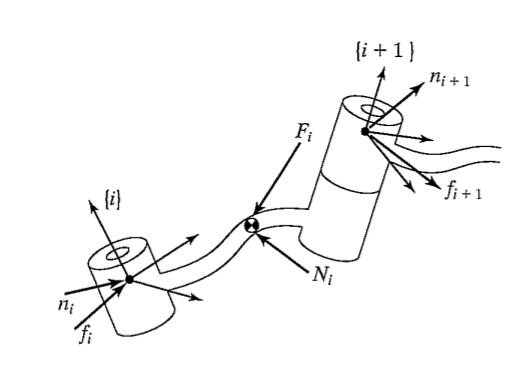
\includegraphics[width=.8\textwidth]{rigidbody/fig/force-balance.png}
    \caption{Διάγραμμα δυνάμεων ισορροπίας}
    \label{fig:force-balance}
\end{figure}

Η πρώτη αναδρομή περιγράφεται από τις εξής σχέσεις για $i : 0 \rightarrow n-1$:

\begin{equation}
    \begin{aligned}
        ^{i+1}\omega_{i+1} = {}^{i+1}R_i \cdot {}^i\omega_i +
        \dot{q}_{i+1} \times {}^{i+1}\hat{Z}_{i+1}\\[10pt]
        ^{i+1}\dot{\omega}_{i+1} = {}^{i+1}R_i \cdot {}^i\dot{\omega}_i +
        {}^{i+1}R_i \cdot {}^i\omega_i \times \dot{q}_{i+1} \cdot
        {}^{i+1}\hat{Z}_{i+1} + \ddot{q}_{i+1} \cdot
        {}^{i+1}\hat{Z}_{i+1}\\[10pt]
        ^{i+1}\dot{u}_{i+1} = {}^{i+1}R_i \cdot (^i\dot{\omega}_i \times
        {}^iP_{i+1} + {}^i\omega_i \times (^i\omega_i \times {}^iP_{i+1}) +
        {}^i\dot{u}_i)\\[10pt]
        ^{i+1}\dot{u}_{C_{i+1}} = {}^{i+1}\dot{\omega}_{i+1} \times
        {}^{i+1}P_{C_{i+1}} + {}^{i+1}\omega_{i+1} \times (^{i+1}\omega_{i+1}
        \times {}^{i+1}P_{C_{i+1}}) + {}^{i+1}\dot{u}_{i+1}\\[10pt]
        ^{i+1}F_{i+1} = m_{i+1} \cdot {}^{i+1}\dot{u}_{C_{i+1}}\\[10pt]
        ^{i+1}N_{i+1} = {}^{C_{i+1}}I_{i+1} \cdot {}^{i+1}\dot{\omega}_{i+1} +
        {}^{i+1}\omega_{i+1} \times {}^{C_{i+1}}I_{i+1} \cdot {}^{i+1}\omega_{i+1}
    \end{aligned}
    \label{equ:iterative-NE-first}
\end{equation}

Η δεύτερη αναδρομή περιγράφεται από τις εξής σχέσεις για $i : n \rightarrow 1$:

\begin{equation}
    \begin{aligned}
        ^if_i = {}^{i}R_{i+1} \cdot {}^{i+1}f_{i+1} + {}^iF_i\\[10pt]
        ^in_i = {}^iN_i + {}^iR_{i+1} \cdot {}^{i+1}n_{i+1} + {}^iP_{C_i} \times
        {}^iF_i + {}^iP_{i+1} \times {}^iR_{i+1} \cdot {}^{i+1}f_{i+1}\\[10pt]
        \tau_i = {}^in^T_i \cdot {}^i\hat{Z}_i
    \end{aligned}
    \label{equ:iterative-NE-second}
\end{equation}



\bibliographystyle{amsplain}
\bibliography{bibliography/bibliography}

\end{document} 